\section{Κατηγορίες χρηστών} \label{section:3-2-user-categories}

Οι χρήστες της πλατφόρμας χωρίζονται σε πρωτεύοντες ή ενεργούς και δευτερεύοντες ή παθητικούς. Πρωτεύοντες χρήστες είναι εκείνοι που εκκινούν διεργασίες στο σύστημα. Δευτερεύοντες είναι οι χρήστες με τους οποίους αλληλεπιδρά το σύστημα αλλά οι ίδιοι δεν εκκινούν διεργασίες σε αυτό. Συνολικά οι χρήστες που συμμετέχουν στο σύστημα είναι οι:

\begin{itemize}
    \item Επισκέπτες
    \item Εγγεγραμμένα μέλη
    \item Δημιουργοί κοινοτήτων
    \item Συμβόλαιο υποκοινότητας
\end{itemize}

\subsection{Ενεργοί χρήστες}

Οι ενεργοί χρήστες στο σύστημα είναι οι επισκέπτες, τα εγγεγραμμένα μέλη και οι δημιουργοί κοινοτήτων.

Όλοι οι χρήστες στο σύστημα είναι αρχικά επισκέπτες. Οι επισκέπτες έχουν τη δυνατότητα να βλέπουν το περιεχόμενο της κοινότητας αλλά δεν μπορούν να συμμετέχουν δημιουργώντας νέο περιεχόμενο (δημοσιεύοντας νέα θέματα ή μηνύματα). Επίσης, δεν μπορούν να συμμετέχουν στις ψηφοφορίες της κοινότητας ή να ψηφίσουν τα μηνύματα.

Όταν ένας επισκέπτης εγγράφεται στο σύστημα, αποκτά έναν μοναδικό, αύξων αριθμό χρήστη και αποτελεί πλέον εγγεγραμμένο μέλος της κοινότητας. Τα εγγεγραμμένα μέλη έχουν τα δικαιώματα των επισκεπτών και μπορούν επιπλέον να προσθέσουν περιεχόμενο στην πλατφόρμα μέσω της δημιουργίας νέων θεμάτων, της δημοσίευσης μηνυμάτων και της ψήφισης στις ψηφοφορίες στις οποίες έχουν δικαίωμα.

Οι δημιουργοί κοινοτήτων είναι οι χρήστες οι οποίοι χρησιμοποιούν την δυνατότητα του συστήματος να δημιουργήσει υποκοινότητες τα μέλη των οποίων διαφοροποιούνται με βάση ένα token. Το token που ορίζει τα μέλη μίας κοινότητας προέρχεται από ένα έξυπνο συμβόλαιο το οποίο ορίζεται κατά τη δημιουργία της κοινότητας. Οι δημιουργοί κοινοτήτων πρέπει να είναι εγγεγραμμένα μέλη της κοινότητας. Ένας δημιουργός κοινότητας δεν έχει παραπάνω δικαιώματα από αυτά των απλών εγγεγραμμένων χρηστών.

\subsection{Παθητικοί χρήστες}

Παθητικοί χρήστες τους συστήματος είναι τα συμβόλαια των υποκοινοτήτων. Τα συμβόλαια αυτά δεν εκκινούν διεργασίες στο σύστημα και δεν αλληλεπιδρούν με αυτό άμεσα. Ωστόσο, μέσω της διάθεσης των token της υποκοινότητας στην οποία χρησιμοποιούνται ορίζουν τους χρήστες της υποκοινότητας αυτής. Συγκεκριμένα, μέσω του διαμοιρασμού των token καθορίζουν ποιοι χρήστες της πλατφόρμας έχουν δικαίωμα ψήφου στις ψηφοφορίες που αφορούν την υποκοινότητα.

\subsection{Σύνοψη χρηστών}

Συμπερασματικά προκύπτουν τρεις διακριτές κατηγορίες ενεργών χρηστών με ξεχωριστά δικαιώματα όπως φαίνεται στο παρακάτω σχήμα (σχήμα \ref{figure:3-2-use-categories-diagram}):

\begin{threeparttable}[H]
    \begin{center}
        \begin{tabularx}{\textwidth}{p{2.3cm} X X X X X X X X X}
            \toprule
            \multirow{7}{2.3cm}{Κατηγορία χρήστη} &\multicolumn{9}{c}{Δικαιώματα} \\ [0.5ex]
            & \spheading{70}{6em}{Προβολή θεμάτων} & \spheading{70}{8em}{Προβολή μηνυμάτων} & \spheading{70}{8em}{Προβολή ψηφοφοριών} & \spheading{70}{8em}{Προβολή ψήφων μηνυμάτων} & \spheading{70}{8em}{Δημιουργία θεμάτων} & \spheading{70}{8em}{Δημιουργία μηνυμάτων} & \spheading{70}{8em}{Δημιουργία ψηφοφοριών} & \spheading{70}{8em}{Ψήφιση σε ψηφοφορίες} & \spheading{70}{8em}{Ψήφιση μηνυμάτων} \\ [0.5ex]
            \midrule
            Επισκέπτες & \textcolor{OliveGreen}{\faIcon{check}} & \textcolor{OliveGreen}{\faIcon{check}} & \textcolor{OliveGreen}{\faIcon{check}} & \textcolor{OliveGreen}{\faIcon{check}} & \textcolor{red}{\faIcon{times}} & \textcolor{red}{\faIcon{times}} & \textcolor{red}{\faIcon{times}} & \textcolor{red}{\faIcon{times}} & \textcolor{red}{\faIcon{times}} \\ [0.5ex]
            Εγγεγραμμένα μέλη & \textcolor{OliveGreen}{\faIcon{check}} & \textcolor{OliveGreen}{\faIcon{check}} & \textcolor{OliveGreen}{\faIcon{check}} & \textcolor{OliveGreen}{\faIcon{check}} & \textcolor{OliveGreen}{\faIcon{check}} & \textcolor{OliveGreen}{\faIcon{check}} & \textcolor{OliveGreen}{\faIcon{check}}\tnote{1} & \textcolor{OliveGreen}{\faIcon{check}}\tnote{1} & \textcolor{OliveGreen}{\faIcon{check}} \\ [0.5ex]
            Δημιουργοί κοινοτήτων & \textcolor{OliveGreen}{\faIcon{check}} & \textcolor{OliveGreen}{\faIcon{check}} & \textcolor{OliveGreen}{\faIcon{check}} & \textcolor{OliveGreen}{\faIcon{check}} & \textcolor{OliveGreen}{\faIcon{check}} & \textcolor{OliveGreen}{\faIcon{check}} & \textcolor{OliveGreen}{\faIcon{check}}\tnote{1} & \textcolor{OliveGreen}{\faIcon{check}}\tnote{1} & \textcolor{OliveGreen}{\faIcon{check}} \\ [0.5ex]
            \bottomrule
        \end{tabularx}
        \begin{tablenotes}
            \item[1] \footnotesize{Μόνο στις υποκοινότητες στις οποίες κατέχει το αντίστοιχο token και σε αυτές οι οποίες δεν έχουν ορισμένο token.}
        \end{tablenotes}
    \end{center}
    \caption{Δικαιώματα χρήσης ανά κατηγορία χρήστη.}
    \label{table:3-2-user-category-permissions}
\end{threeparttable}

\begin{figure}[H]
    \centering
    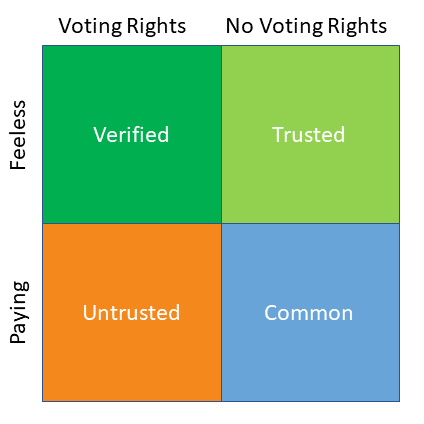
\includegraphics[width=0.6\textwidth]{assets/figures/chapter-3/user_categories}
    \caption{Κατηγορίες χρηστών}
    \label{figure:3-2-use-categories-diagram}
\end{figure}
